\labelsubsection{Results and Observations}{subsec:results_and_observations}
In the next sections we will investigate the questions we posed in the previous chapter.
After that, we will gather our findings to form an judgement of the validity of our hypothesis.

\todo{Observations + possible explanations}
\todo{How do the results relate to hypothesis?}
\todo{Error analysis}
\todo{Comparison between text n-grams and concept maps/co-occurrence graphs}
\todo{Look at concepts used in concept maps: frequency in whole corpus, ...}

\subquestionref{question:structure_diversity}
To investigate whether concept maps are useful for text classification, we first look at the structure of concept maps.
Our hypothesis especially highlights the structure of the concept maps since it is one of the main differences to other text representation.
Finding out whether the structure of concept maps is heterogeneous therefore is a first crucial step.

In Figure \ref{fig:graph_statistics}, we gathered metrics about the connectedness of concept maps and co-occurrence graphs with window size 1 for comparison.
One thing that immediately becomes apparent is the compression factor of the concept maps: on average, only approximately 8\% of the original text-content is retained in the concept maps.
This compression is useful for tasks like text summarization where only important concepts should be kept from the underlying text.

One consequence of the compression can be seen when looking at the connectedness of the concept maps.
On average, concept maps only have 1.36 edges per node. The minimum number of edges per node is 1 since we removed all unconnected nodes.
So, concept maps do not only have few nodes, because of the compression, but also a relatively low number of edges between them.
This is most likely due to the small length of the underlying texts.
The shortness of the text results in a lower number of occurrences of some concept in the text, ie. most of the concepts occur only once in a text.
To address this issue, we then searched for a dataset with longer texts per document.

\begin{figure}[ht]
	\centering
	\begin{tabular}{lcccccc}
		{} &  \multicolumn{2}{c}{\#nodes/\#words} &  \multicolumn{2}{c}{\#edges/\#nodes} & \multicolumn{2}{c}{\#nodes/graph} \\
		{} & concept map &  co-occurrence & concept map & co-occurrence & concept map & co-occurrence\\
		\midrule
		ling-spam       & 0.05 & 0.23 & 1.32 & 2.86 & 45.95 & 4.11 \\
		ng20            & 0.05 & 0.18 & 1.38 & 2.71 & 584.63 & 87.52 \\
		reuters-21578   & 0.09 & 0.21 & 1.46 & 2.86 & 63.07 & 13.20 \\
		review\_polarity & 0.08 & 0.20 & 1.42 & 2.67 & 50.36 & 10.55 \\
		rotten\_imdb     & 0.09 & 0.30 & 1.22 & 1.70 & 52.09 & 11.23 \\
		tagmynews       & 0.13 & 0.37 & 1.30 & 1.81 & 52.74 & 13.25 \\
		webkb           & 0.05 & 0.22 & 1.39 & 3.01 & 55.69 & 5.36 \\
		\midrule
		\O{}            & 0.08 & 0.24 & 1.36 & 2.52 & 129.22 & 20.75 \\
		\bottomrule
	\end{tabular}
	\caption{Graph statistics. \textit{\#words} is the number of words in the whole text dataset. The \textit{\#edges/\#nodes} metric is for the co-occurrence graphs with a window size of 1. The \textit{\#nodes/\#words} metric is a compression factor. Note that, on average, the concept maps have a compression factor of 8\% compared to the 24\% of the co-occurrence graph. This means that co-occurrence graphs have approximately three times more content than concept maps. The \textit{\#edges/\#nodes} metric is an indicator for the connectedness of the graphs. Because we remove nodes which have no edge to other nodes, the \textit{\#edges/\#nodes} metric captures the average degree of the nodes. Looking at that metric we also see that, on average, the co-occurrence graphs with window size 1 have roughly twice as much edges per node as concept maps.}\label{fig:graph_statistics}
\end{figure}

\todo{New dataset! Statistics}
\todo{Add statistics about \# of occurrences of concepts in graphs}

Another hint for the un-connectedness of concept maps is the number of connected components.
In Figure \ref{fig:percentage_more_than_one_connected_component} we can see that most of the graphs have more than one connected component. Together with the observation of the low number of nodes per graph, this also implies the low connectedness of concept maps.
In Figure \ref{fig:histogram_connected_components} we also plotted the histogram of the number of connected components per graph.

In Figure \ref{fig:graph_examples} shows examples of concept maps and co-occurrence graphs with different window sizes.

\begin{figure}[ht]
\centering
\centering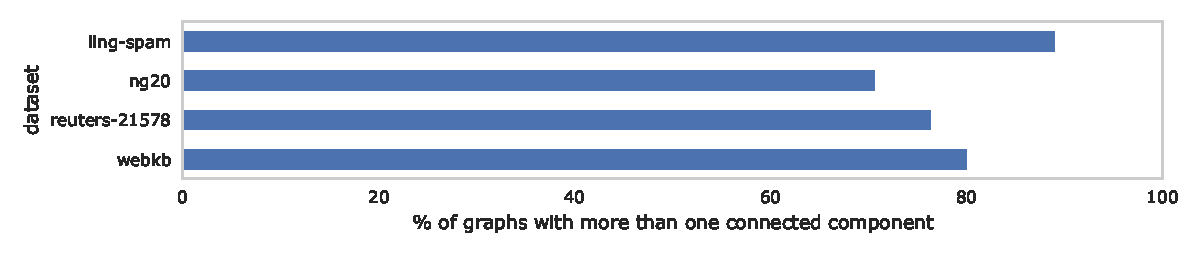
\includegraphics[width=1\linewidth]{assets/figures/percentage_more_than_one_connected_component.pdf}
\caption{Percentage of graphs with more than one connected component. TODO: This can also be put into a table!}\label{fig:percentage_more_than_one_connected_component}
\end{figure}

\begin{figure}[ht]
\centering
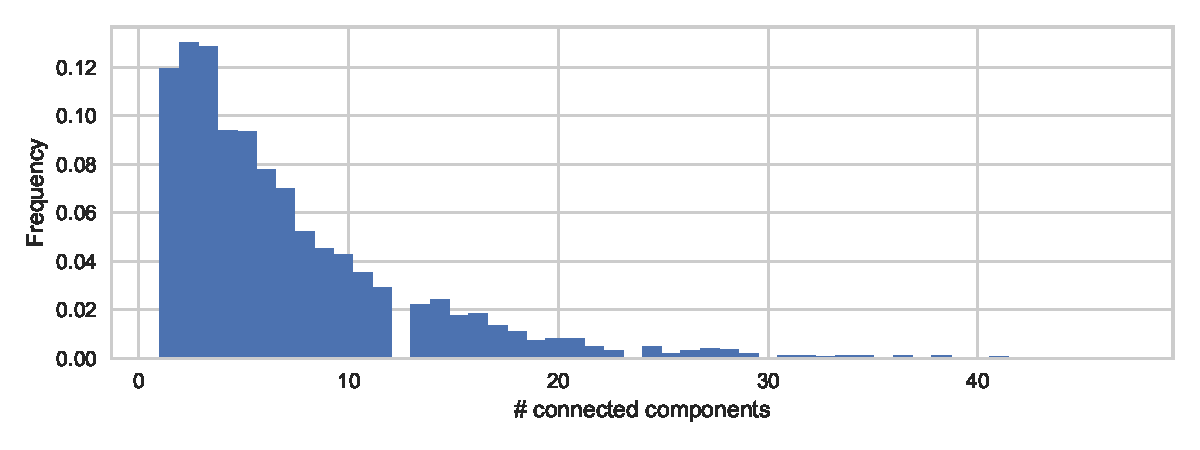
\includegraphics[width=0.8\linewidth]{assets/figures/hist-connected-components-ling-spam-CMap.pdf}
\caption{Histogram of connected components per concept map. From \textit{ling-spam} dataset.}\label{fig:histogram_connected_components}
\end{figure}

\begin{figure}[ht]
\centering
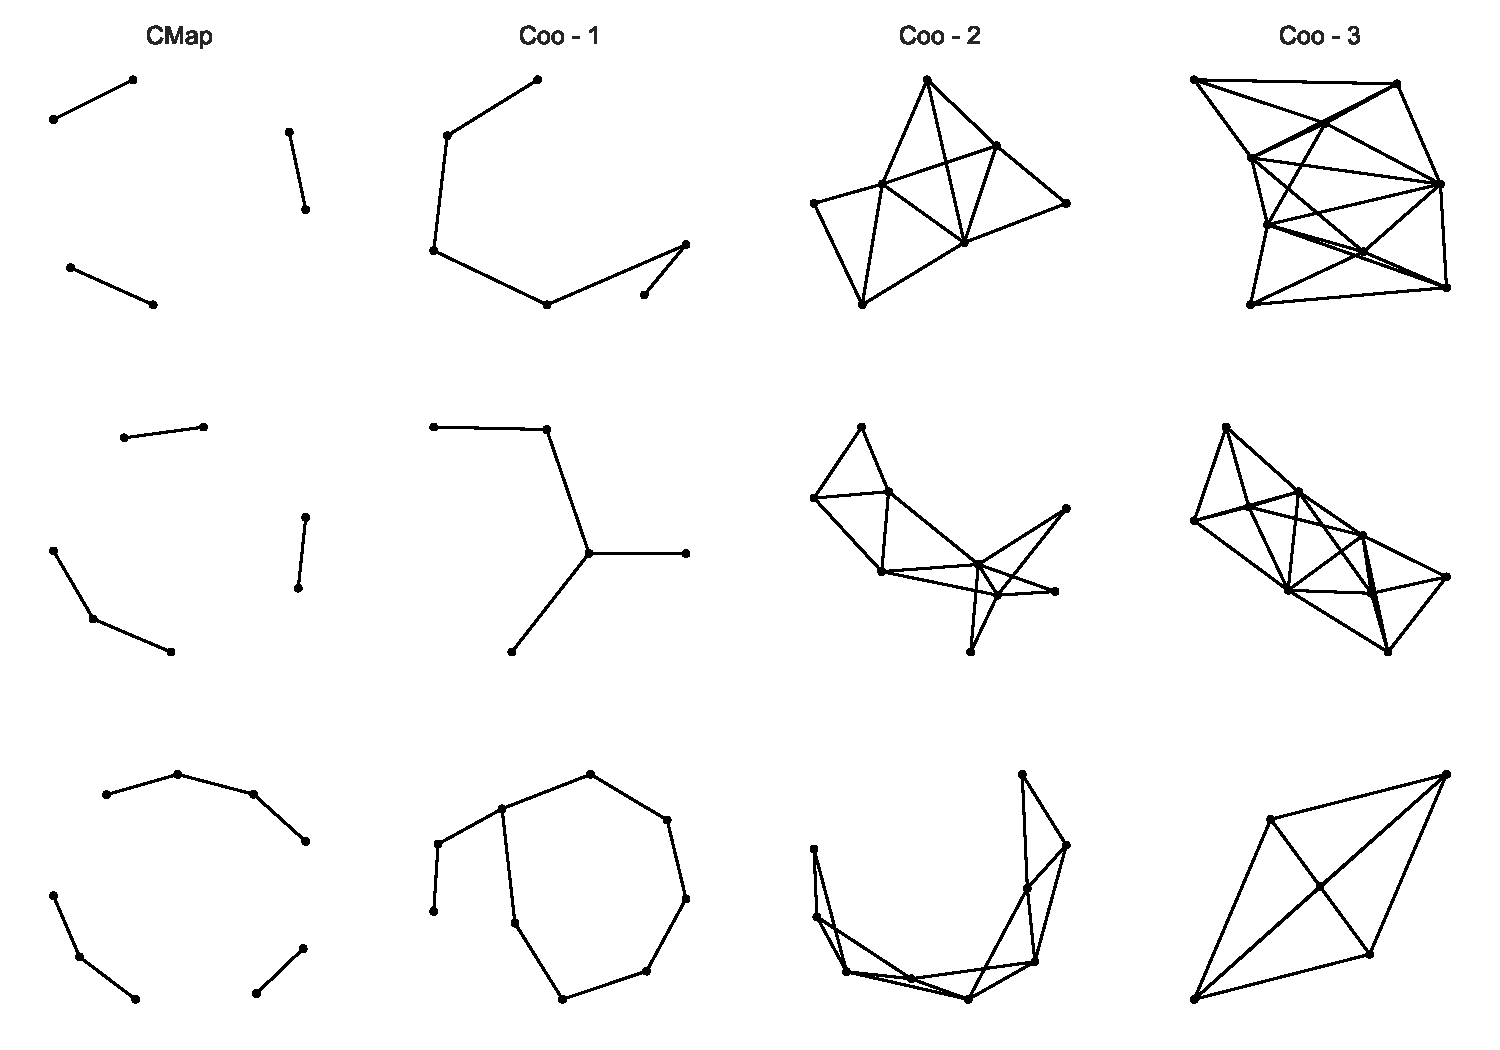
\includegraphics[width=0.6\linewidth]{assets/figures/graph-examples.pdf}
\caption{Graph examples per type. Three examples are shown per type. The number after the co-occurrence graph label signify the window size. The concept map examples all have more than one connected component, while the co-occurrence graphs all have only one. Taken from the \textit{ling-spam} dataset.}\label{fig:graph_examples}
\end{figure}

\begin{figure}[ht]
\centering
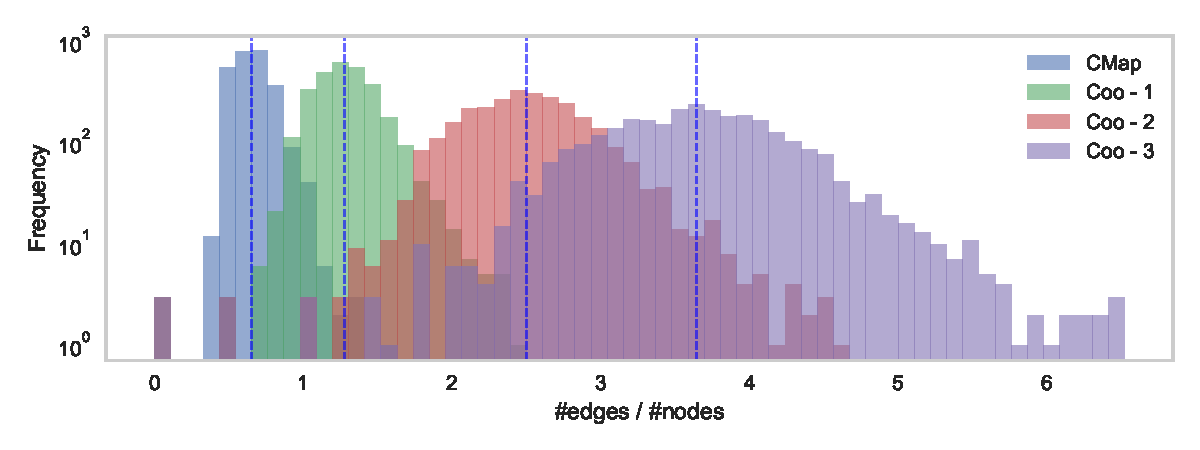
\includegraphics[width=0.7\linewidth]{assets/figures/hist-edgesnodes.pdf}
\caption{Histogram of the number of edges divided by the number of nodes. Per graph type. The lines correspond to the median value.}
\label{fig:histogram-edges-div-nodes-per-type}
\end{figure}

The co-occurrence graphs also have a simple structure.
Co-occurrence graphs are always connected, ie. the number of connected components is 1, or 0 in the case of an empty graph.
When the window size is 1, the graph is similar to a path, meaning that most of the nodes have a degree $< 2$. With increasing window size, the graph also gets more connected.

\subquestionref{question:importance_structure}
After investigating the structure of concept maps, we now aim to quantify the importance of the structure compared to the content.
The content, that is the node and edge labels, of concept maps are also captured in co-occurrence graphs and with conventional text-based approaches. So, the next interesting question about concept maps is, how much or whether the structure adds to the classification performance.
For this, we compare the results of using graph kernels which use \textbf{(a)} only the content, \textbf{(b)} only the structure and \textbf{(c)} both content and structure.

For \textbf{(a)} (content only), we use a kernel that discards all edges and uses only the labels of nodes and edges. Next, we create a bag-of-words vector representation out of the labels and edges.
In this step, we also evaluated using not only single words and counting them, but also using word n-grams of size 2, or bigrams.
For this, we create pairs of words by joining node labels together that have an edge between them.
The resulting vector representations of the graph then get fed into a conventional classifier, in our case a SVM.

For \textbf{(b)} (structure only), we use a modified version of the Weisfeiler-Lehman graph kernel. Before applying the actual WL kernel, we discard all node labels and give every node in all graphs the same label, effectively ridding the graphs of content. Next, we apply the WL graph kernel. This variant of WL only takes the structure of the graph into account.
After executing WL on the graphs, we obtain the feature maps which get subsequently get fed into a SVM also.

For \textbf{(c)} (structure and content combined), we use the Weisfeiler-Lehman that takes both structure and content into account.

In Table \ref{fig:table-results-structure-vs-content} we report the results obtained from these experiments.

\begin{figure}[ht]
\centering
\begin{tabular}{llrrr}
          & & \multicolumn{3}{c}{f1 macro} \\
Dataset & Type & \textbf{(a)} content only & \textbf{(b)} structure only & \textbf{(c)} combined\\
\midrule
ling-spam & concept map &  0.933020 &  0.468187 &  0.741138 \\
          & cooccurrence &  0.959041 &  0.519897 &  0.794719 \\
\midrule
ng20 & concept map &  0.592340 &  0.035334 &  0.263055 \\
          & cooccurrence &  0.679036 &  0.049227 &  0.511980 \\
\midrule
reuters-21578 & concept map &  0.241263 &  0.005962 &  0.085752 \\
          & cooccurrence &  0.293941 &  0.012733 &  0.229710 \\
\midrule
webkb & concept map &  0.472472 &  0.162010 &  0.222296 \\
          & cooccurrence &  0.714741 &  0.170633 &  0.472485 \\
\bottomrule
\end{tabular}
\caption{Comparison of linearized graph with CountVectorizer and results of WL}\label{fig:table-results-structure-vs-content}
\end{figure}

\todo{Interpret results!}
\todo{Ratio between (a), (b) to (c). Why is combined less good?}
\todo{Why do we not use the zero-th iteration, ie. counting the plain labels?}


\subquestionref{question:comparison_coo}

\todo{Co-occurrence:"Text kernel" performs nearly as well as normal text}
\todo{Co-occurrence: only minor decrease (1\%) in performance when only using nouns}
\begin{figure}[ht]
\centering
\begin{tabular}{lrrr}
&  concept\_map &  cooccurrence &   ratio \\
\midrule
ling-spam       &  0.7165 &  0.9112 &  0.7863 \\
ng20            &  0.2904 &  0.3964 &  0.7325 \\
review\_polarity &  0.5615 &  0.6656 &  0.8436 \\
rotten\_imdb     &  0.5786 &  0.8070 &  0.7170 \\
webkb           &  0.2763 &  0.5082 &  0.5438 \\
\bottomrule
\end{tabular}
\caption{Comparison of co-occurrence results with concept maps}
\end{figure}

\subquestionref{question:comparison_text}
As one can see in Figure \ref{fig:results_cmap_vs_text}, the text-only- outperform graph-only approaches by a high margin.
This is most likely due to the high compression factor of concept maps and co-occurrence graphs.

\begin{figure}[ht]
\centering
\missingfigure[figcolor=white]{}
\caption{Comparison of concept maps with text}
\label{fig:results_cmap_vs_text}
\end{figure}

\subquestionref{question:dataset_diversity}
\todo{WL sparsity per dataset}

\subquestionref{question:comparison_combined}
As we have seen in the results of the last section, text-based approaches outperform graph-only approaches.
In this section we investigate how and whether the graph-based approaches improve the classification score when combined with text-based approaches.

For the text features we vectorized the text with a bag-of-words approach. We also tried features with tfidf.
For the graph features we used the Weisfeiler-Lehman algorithm since it is able to create feature map $\phi(G)$ for the graphs.
These feature maps can easily be concatenated with the text features.
For other graph kernels where an explicit feature map $\phi(G)$ can not be calculated, in order to combine graph- and text features, we would have had to create a combined kernel that takes into account both text- and graph features and returns a gram matrix for both of them.
The interpretability of this approach would be far lower since both graph- and text-features would be merged without being able to distinguish the relative importance of the text- and graph features after creating the gram matrix.

In Figure \ref{fig:results_comparison_combined} we see the classification scores for the combined features for both co-occurrence graphs and concept maps.

\todo{This is not true anymore. Classification performance on test set is different!}
As we see, the performance of the combined approached compared the text-only approach is comparable.
With some datasets, the combined approach is slightly better than the text-only approach. Especially for the ng20 dataset, we see an improvement of ca. 3\% over the text-only approach.
To test whether this difference in performance is due to chance, we used the permutation test, 

To better understand the performance when combined text- and graph features, we also trained a one-layer neural network with the combined features and after training, we looked at the weights in the first layer.
The weights, or coefficients, are an indicator for the importance of a input feature.
Thus we can look at the weights for the text features and compare them to the weights for the graph features.
This gives an insight into the relative importance of text- and graph features.

\todo{SVM trained on combined, coefficients}
\todo{Analysis of coefficients}


\begin{figure}[ht]
\centering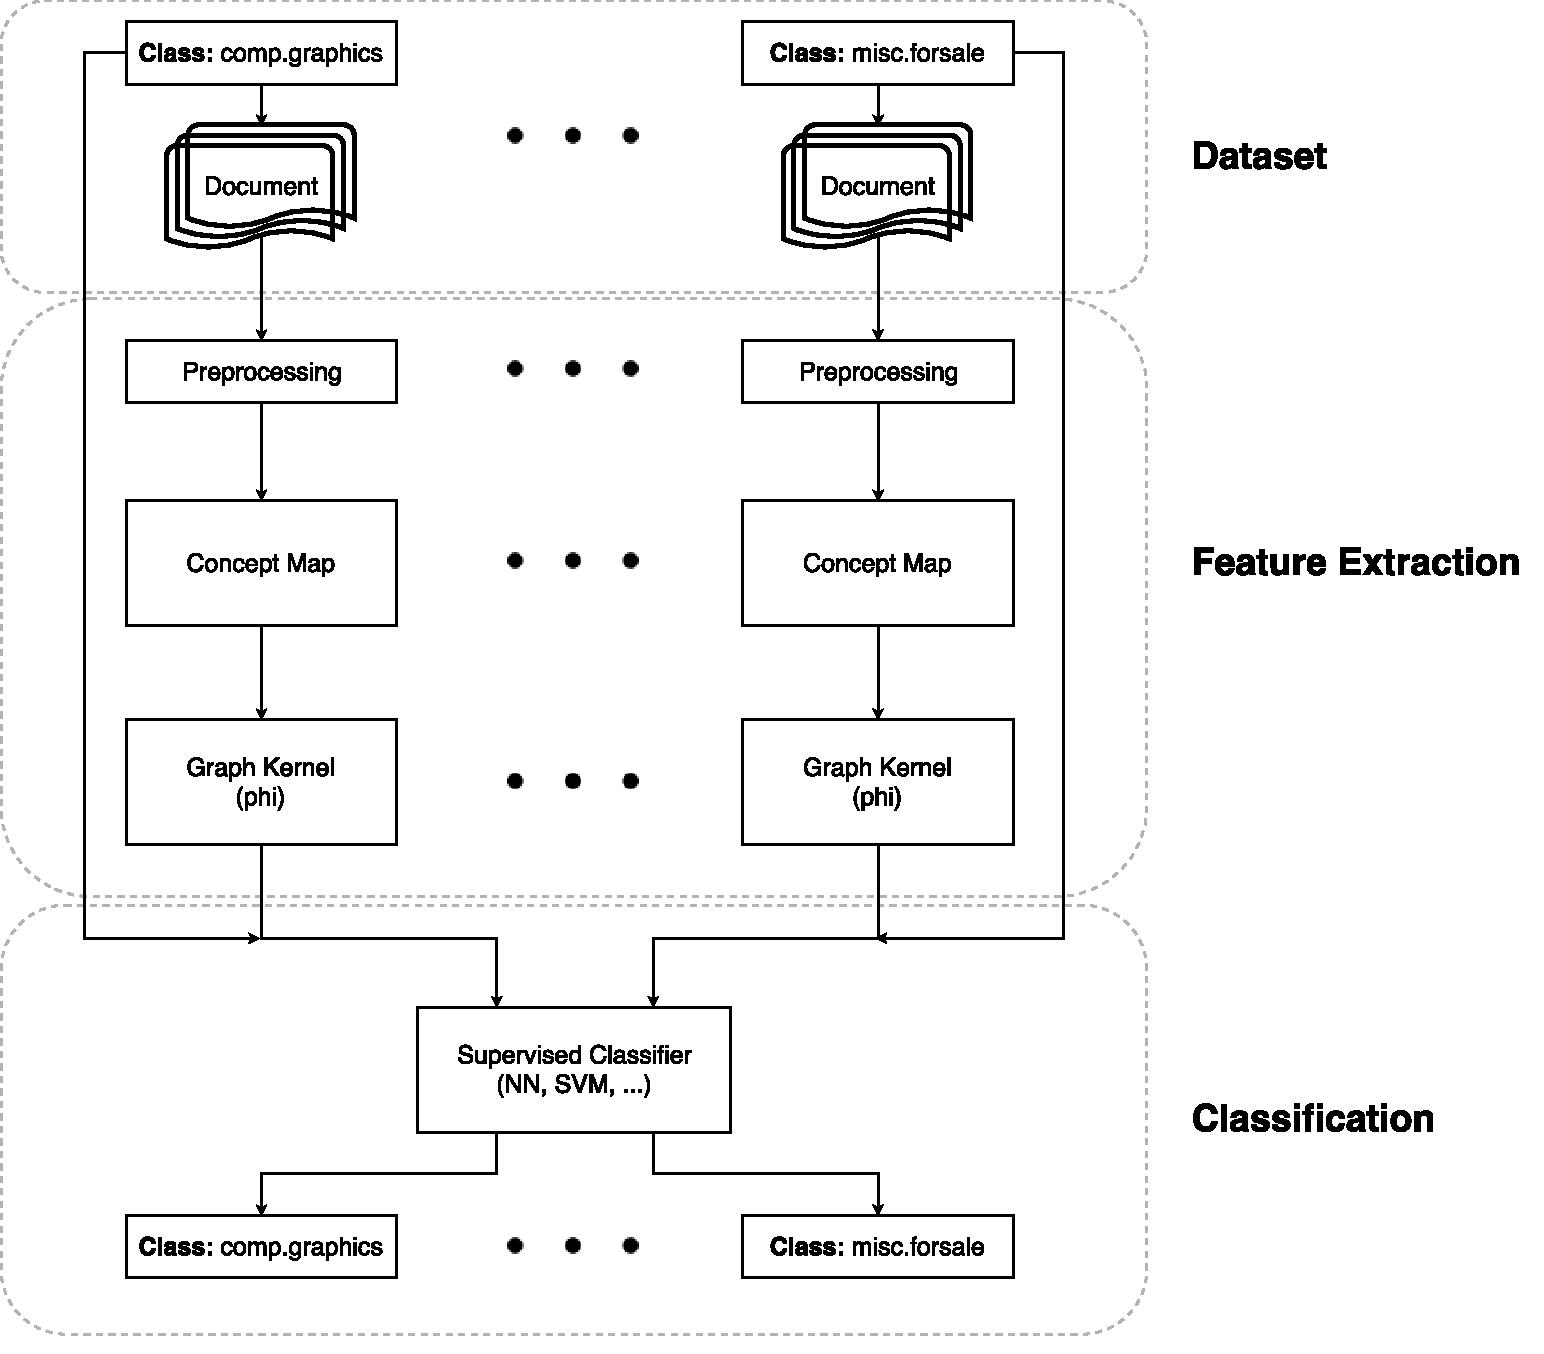
\includegraphics[width=0.6\linewidth]{assets/figures/approach.pdf}
\caption{Histogram of SVM coefficients trained on combined features}
\end{figure}

\begin{figure}[ht]
\centering
\begin{tabular}{lrr}
\toprule
 &  concept-map &  cooccurrence \\
\midrule
ling-spam       &  0.0897 &  0.0651 \\
ng20            &  0.0508 &  0.0457 \\
reuters-21578   &  0.0899 &  0.0131 \\
review\_polarity &  0.1848 &  0.0323 \\
rotten\_imdb     &  0.1731 &  0.0801 \\
tagmynews       &  0.1399 &  0.0229 \\
webkb           &  0.1132 &  0.0526 \\
\bottomrule
\end{tabular}\caption{Percentage of concepts that occur only once in the dataset. Per graph type and dataset.}
\end{figure}

\begin{figure}[ht]
\centering
\begin{tabular}{llcc}
  &  & \multicolumn{2}{c}{Graph type} \\
   dataset   & &  Concept Map &  Co-Occurrence \\
\midrule
ling-spam 
          & text only & \multicolumn{2}{c}{ 0.966179 }\\
          & graph only &  0.741138 &  0.794719\\
          & combined &  0.986928 &  0.977104\\
\midrule
ng20 
          & text only & \multicolumn{2}{c}{ 0.681245 }\\
          & graph only &  0.263055 &  0.511980\\
          & combined &  0.738239 &  0.690968\\
\midrule
reuters-21578 
          & text only & \multicolumn{2}{c}{ 0.320838 }\\
          & graph only &  0.085752 &  0.229710\\
          & combined &  0.264947 &  0.291086\\
\midrule
webkb 
          & text only & \multicolumn{2}{c}{ 0.702095 }\\
          & graph only &  0.222296 &  0.472485\\
          & combined &  0.722667 &  0.741964\\
\bottomrule
\end{tabular}
\caption{Comparison of classification using both concept maps and text. TODO: Add standard deviations}%
\label{fig:results_comparison_combined}
\end{figure}

\labelsubsection{Related And Intermediate Observations}{subsec:related_and_intermediate_observation}

\todo{Sparsity of feature vectors}
\todo{Complexity of approach}
\todo{Usefulness of WL to get feeling for graph connectedness, uniqueness of structure, uniqueness of labels}

\subsubsection{Weisfeiler-Lehman extension}
With increasing iterations $h$ of the Weisfeiler-Lehman algorithm, the exact matches of the subtrees of height $h$ become much more improbable.
In iteration 0, the Weisfeiler-Lehman only counts the number of node labels in the graphs, for iteration 1 it takes the immediate neighbourhood of the nodes into account, for iteration 2 is takes the neighbourhood of the neighbourhood into account and so on.
So, with \textbf{(1)} higher iterations, the probability of having an exact match decreases.

Another difficulty arises for nodes with a high number of neighbours. \textbf{(2)} The probability of an exact match also decreases with a higher degree.

These two difficulties, \textbf{(1)} the increased difficulty of a match with higher iterations and \textbf{(2)} the increased difficulty of a match for nodes with higher degrees, are not addressed when using Weisfeiler-Lehman in its plain version. Both difficulties are neither encoded in the features maps nor when creating the gram matrix.

As a possible solution for these difficulties, we propose an extension to the plain Weisfeiler-Lehman algorithm.
Our extension augments the WL algorithm by adding node weights.
For each of the nodes in all graphs, we first calculate node weights which encode the importance of the nodes or the difficulty of getting an exact match in WL.
An example of such node weights are the node degree or node weights extracted with PageRank.
The node degree is an interesting metric for node weights since it actually encodes the size of the immediate neighbourhood of a node and therefore could possibly address both problem \textbf{(1)} and \textbf{(2)}.

\todo{Explain how to actually use the node weights.}
\todo{Remark that the node weights could be seen as an additional metric of frequency: nodes with a higher degree have been in the text more frequently.}

Our other extension to the WL algorithm addresses problem \textbf{(1)}, the difficulty of having a match when the iteration increases.
To solve this difficulty, we propose weighting the features of each iteration.
The feature maps of WL consist of the concatenated feature maps for each iteration.
For this extension, we propose weighting the feature maps of each iteration $h$ by a factor given by a function $f(h)$.
So, for a feature map, $\phi(G)$, of a graph $G$ for $h=2$ iterations, the feature map can be decomposed into the feature maps of each of the two $h$ iterations:
\begin{equation*}
\phi(G)=(\phi_{h=1}(G), \phi_{h=2}(G))
\end{equation*}
We now propose to weight the individual feature maps by the factor determined by function $f(h)$, so:
\begin{equation*}
\phi_{f}(G)=(f(1) \cdot \phi_{h=1}(G), f(2) \cdot \phi_{h=2}(G))
\end{equation*}
So, basically the function $f(h)$ works as a decaying factor to decreasing iterations $h$.
When the function $f(h)$ increasing (steigend?), the increasing importance with higher iterations is encoded into the resulting feature map $\phi_f(G)$.

\todo{This is NOT a solution when feature-scaling is done.}